% ============================================================================
% CHAPTER 2 -- REQUIREMENTS SPECIFICATION
% End-of-Study Report -- MES-X Dependency Traceability System
% ============================================================================

\chapter{Requirements Specification}
\label{chap:requirements}

% ----------------------------------------------------------------------------
\section{Introduction}
\label{sec:req-intro}

Requirements specification is the point where the system is described in clear,
technology-independent terms. Before any architecture is proposed or any code
is written, the team needs an agreed description of what the system must do and
which quality attributes it must preserve. That specification then becomes the
baseline for design and for later validation.

This chapter presents the requirements for the MES-X Dependency Management
system. The requirements were derived by examining the manual traceability
process described in the previous chapter, with attention to the artifacts used,
the steps followed by practitioners, the recurring errors, and the decisions
that need to be supported. The analysis was informed by discussions with
release engineers and developers in the MES X.0 division and by observation of
the existing workflow.

The chapter is organized as follows. Section~\ref{sec:functional-requirements}
describes the functional requirements, Section~\ref{sec:nonfunctional-requirements}
covers the non-functional requirements, and Section~\ref{sec:use-case-model}
presents the use case model. The chapter ends with a short conclusion that
connects the requirements to the architecture introduced later.

% ----------------------------------------------------------------------------
\section{Functional Requirements}
\label{sec:functional-requirements}

Functional requirements describe the behavior the system must provide from the
user and process perspective. They define the capabilities needed to trace
artifacts across work items, pull requests, commits, and tags.

% ----------------------------------------------------------------------------
\section{Work Item Traceability Requirements}
\label{sec:req-work-items}

Work items are the usual starting point for traceability analysis. They express
the needs, tasks, and user stories that define the expected behavior of the
software, and they serve as the roots for the dependency graph.

\begin{itemize}
  \item \textbf{FR-WI-01 -- Single Work Item Retrieval}: The system must be able to retrieve a work item from Azure DevOps by its numeric identifier and return a normalized view of its metadata, including title, type, state, assignee, and all relation links.

  \item \textbf{FR-WI-02 -- Relation Type Interpretation}: The system must be able to interpret the relation types used by Azure DevOps work items, including parent-child links, peer links, and artifact links to external objects such as pull requests. Each relation type must be handled correctly during graph construction.

  \item \textbf{FR-WI-03 -- Dependency Graph Traversal}: The system must be able to explore the full dependency graph reachable from a root work item by following relation links across all hierarchy levels. The traversal must be cycle-safe and must support graphs of arbitrary depth without affecting correctness.

  \item \textbf{FR-WI-04 -- Multi-Root Batch Analysis}: The system must be able to accept several work item identifiers as the starting points of one analysis session, traverse the graph for each root, and return one aggregated and deduplicated result covering all reachable work items.

  \item \textbf{FR-WI-05 -- Pull Request Reference Extraction}: While traversing work item relations, the system must identify and extract all references to associated pull requests, producing a deduplicated list of pull request identifiers for later resolution.

  \item \textbf{FR-WI-06 -- Progressive Streaming for Large Datasets}: For analysis sessions involving many work items, the system must support a progressive delivery mode in which partial results are streamed to the client as they are discovered, so the user can follow progress in real time instead of waiting for the full traversal to finish.
\end{itemize}

% ----------------------------------------------------------------------------
\section{Pull Request Traceability Requirements}
\label{sec:req-pull-requests}

Pull requests form the bridge between work tracking and source control. They are
the point where implementation work becomes a formal change set in Azure
DevOps, so the system must resolve them accurately and enrich them with useful
context.

\begin{itemize}
  \item \textbf{FR-PR-01 -- Pull Request Metadata Resolution}: The system must be able to retrieve the full metadata of a pull request from the Azure DevOps Git API using its identifier, including title, status, source and target branches, and the repository identifier.

  \item \textbf{FR-PR-02 -- Linked Work Item Retrieval}: The system must be able to retrieve the work items formally linked to a pull request on the Git side of Azure DevOps. This list may differ from the work items linked from the work-tracking side, and both views must be supported.

  \item \textbf{FR-PR-03 -- Repository Identity Propagation}: For each resolved pull request, the system must extract and propagate the repository name so that downstream components can group and classify results without making additional API calls.

  \item \textbf{FR-PR-04 -- Traceability Chain Bridging}: The system must use resolved pull request information to extend the traceability chain from work items into source control. PR resolution must produce the structured context needed for commit and tag resolution.
\end{itemize}

% ----------------------------------------------------------------------------
\section{Commit Traceability Requirements}
\label{sec:req-commits}

Commits are the most detailed part of the traceability chain. They capture the
actual code changes behind a requirement and provide the context needed to
relate those changes to branches and release tags.

\begin{itemize}
  \item \textbf{FR-CO-01 -- Commit Resolution via Pull Request}: The system must be able to retrieve the commits merged as part of a specific pull request using the Azure DevOps Git API. This is the main path from work items to code changes when a formal PR flow was used.

  \item \textbf{FR-CO-02 -- Commit Resolution via Work Item}: The system must be able to retrieve commits directly linked to a work item through Azure DevOps relation metadata, independently of any pull request.

  \item \textbf{FR-CO-03 -- Commit Deduplication}: When the same commit is reachable through multiple paths, such as a direct work item link and a pull request link, the system must keep only one instance in the final result. Deduplication must happen by commit identifier before downstream processing.

  \item \textbf{FR-CO-04 -- Branch Context Resolution}: For a given repository and commit reference, the system must be able to retrieve the branch references that contain the commit, so the development stream can be identified.

  \item \textbf{FR-CO-05 -- Tag Context Resolution}: For a given repository and commit reference, the system must be able to identify the repository tags associated with the commit, specifically the most recent tag reachable from the commit on the relevant branch. This tag context is the main input for release classification.

  \item \textbf{FR-CO-06 -- Batch Tag Resolution}: The system must support a batch mode for tag resolution in which the tag context of several commits in the same repository is resolved in a single API interaction. This is necessary to keep performance acceptable on large graphs.
\end{itemize}

% ----------------------------------------------------------------------------
\section{Data Aggregation Requirements}
\label{sec:req-aggregation}

Aggregation requirements govern how the system consolidates the data collected
across the traceability pipeline. The goal is to produce one coherent result
that is normalized, deduplicated, and suitable for both automated use and human
review.

\begin{itemize}
  \item \textbf{FR-AG-01 -- Cross-Domain Result Consolidation}: The system must consolidate the normalized results from work item traversal, pull request resolution, commit resolution, and tag enrichment into one unified data structure representing the complete dependency view.

  \item \textbf{FR-AG-02 -- Global Deduplication}: During consolidation, the system must remove duplicate work items, pull request references, and commit identifiers that arise from multi-path traversal. Each entity must appear only once in the final result.

  \item \textbf{FR-AG-03 -- Referential Consistency}: The aggregated result must remain internally consistent. Every pull request reference must correspond to a resolved PR record, every commit reference must correspond to a commit record, and every repository name must be used consistently across the result.

  \item \textbf{FR-AG-04 -- Decision Classification}: The system must apply a classification rule to the aggregated trace data that groups work items by completion state and repositories into release-relative decision buckets based on commit tag context. The output must be ready for release-readiness assessment without additional manual interpretation.

  \item \textbf{FR-AG-05 -- Structured Output Format}: All aggregated outputs must be returned as typed, structured responses that follow documented data contracts. The output structure must be stable, versioned, and independent of internal implementation details.
\end{itemize}

% ----------------------------------------------------------------------------
\section{Analysis and Reporting Requirements}
\label{sec:req-analysis}

The system is not only a retrieval tool. It must also turn traceability data
into something that helps people make decisions about scope, integration, and
release readiness.

\begin{itemize}
  \item \textbf{FR-AN-01 -- Dependency Relationship Identification}: The system must explicitly expose the relationships between development artifacts at every level of the chain: which work items are related to which other work items, which pull requests are associated with which work items, and which commits are associated with which pull requests and repositories.

  \item \textbf{FR-AN-02 -- Repository-Based Grouping}: The system must be able to group resolved commits and pull requests by repository, producing a per-repository view of the changes associated with the analyzed work items. This is important for release engineers who work service by service.

  \item \textbf{FR-AN-03 -- Release Context Interpretation}: The system must interpret the tag context of each commit to determine its position relative to a release boundary, classifying it as preceding, following, or straddling a specified release tag. The interpretation must be applied consistently across all repositories.

  \item \textbf{FR-AN-04 -- Multi-Level Traceability View}: The system must produce a complete traceability view across all relevant abstraction levels: epics and features, user stories and tasks, pull requests, commits, and repository tags. This full-chain view must be available in a single analysis session.

  \item \textbf{FR-AN-05 -- Read-Only Operation}: All system operations must be read-only with respect to Azure DevOps. The system must not create, modify, or delete any artifact in Azure DevOps under any circumstances.
\end{itemize}

% ----------------------------------------------------------------------------
\section{Non-Functional Requirements}
\label{sec:nonfunctional-requirements}

Non-functional requirements define the quality attributes the system must meet
to be suitable for use in the Forvia industrial environment. They constrain how
the functional requirements are delivered, with attention to performance,
scalability, reliability, security, and maintainability.

% ----------------------------------------------------------------------------
\section{Performance Requirements}
\label{sec:req-performance}

Performance is a core concern because the system is meant to replace a slow
manual process. If the automated version is not clearly faster, adoption will be
limited even if the functional behavior is correct.

\begin{itemize}
  \item \textbf{NFR-PE-01 -- Analysis Response Time}: For single work item trace operations involving a dependency graph of typical size, up to thirty related work items across two or three hierarchy levels, the system must return a complete result within a response time that is practical for interactive use.

  \item \textbf{NFR-PE-02 -- Batch Processing Efficiency}: For batch analysis sessions involving multiple work item roots, the system must complete processing in a time that grows sub-linearly with the number of roots, using parallel execution and shared caching of common subgraphs.

  \item \textbf{NFR-PE-03 -- API Call Minimization}: The system must minimize the number of API calls issued to Azure DevOps for a given analysis session by using batch requests, caching, and deduplication. Unnecessary calls are not acceptable, both for performance and for rate-limit protection.

  \item \textbf{NFR-PE-04 -- Responsive User Feedback}: For operations that take more than a few seconds, the system must provide continuous progress feedback through progressive streaming so the interface stays responsive and informative.
\end{itemize}

% ----------------------------------------------------------------------------
\section{Scalability Requirements}
\label{sec:req-scalability}

The MES X.0 platform continues to grow. New microservices are added, existing
services expand, and the number of development artifacts increases over time.
The traceability system must remain usable as that growth continues.

\begin{itemize}
  \item \textbf{NFR-SC-01 -- Work Item Volume Scalability}: The system must remain functional and performant as the number of work items in the analyzed Azure DevOps project grows, without requiring changes to the core traversal or resolution logic.

  \item \textbf{NFR-SC-02 -- Repository and Service Count Scalability}: The system must handle dependency graphs that span more repositories and microservices over time, while keeping commit and tag resolution efficient through batch processing.

  \item \textbf{NFR-SC-03 -- Extensibility for New Artifact Types}: The architecture must allow future additions, such as pipeline run artifacts, automated test results, or release deployment records, without forcing a redesign of the current components or their data contracts.

  \item \textbf{NFR-SC-04 -- Configuration-Driven Adaptability}: System behavior that is likely to vary across environments, such as the Azure DevOps organization, project identifiers, or API credentials, must be externalized into configuration so the system can be deployed in different contexts without code changes.
\end{itemize}

% ----------------------------------------------------------------------------
\section{Reliability Requirements}
\label{sec:req-reliability}

In an industrial setting, users need to trust the result. If analysis outputs are
inconsistent or fragile, people will fall back to manual verification and lose
the benefit of the system.

\begin{itemize}
  \item \textbf{NFR-RE-01 -- Result Determinism}: Given identical inputs and the same Azure DevOps state, the system must produce identical results across successive analysis sessions. Non-deterministic behavior caused by race conditions, unordered concurrent results, or non-reproducible data access is not acceptable.

  \item \textbf{NFR-RE-02 -- Partial Failure Isolation}: If some Azure DevOps API calls fail during analysis because of transient network errors, rate limiting, or partial unavailability, the system must isolate the failure to the affected subset and continue processing the rest of the analysis. Partial failures must be reported clearly and must not silently corrupt the result.

  \item \textbf{NFR-RE-03 -- Data Integrity Preservation}: Throughout the traceability pipeline, the system must preserve the integrity of the data it processes. Entity identifiers, relation links, and commit references must remain accurate and unchanged from retrieval through normalization, aggregation, and final output.

  \item \textbf{NFR-RE-04 -- Transient Error Recovery}: For external API calls that fail with transient errors such as timeouts or temporary service unavailability, the system must implement a structured retry mechanism before reporting failure to the caller.
\end{itemize}

% ----------------------------------------------------------------------------
\section{Maintainability Requirements}
\label{sec:req-maintainability}

The system is expected to stay in use and evolve with the MES X.0 platform.
Maintainability therefore matters over the long term: the code must remain easy
to understand, change, and extend by engineers who did not build the first
version.

\begin{itemize}
  \item \textbf{NFR-MA-01 -- Modular Component Structure}: The system must be organized into cohesive modules with clear responsibilities. Each module must be understandable and testable on its own.

  \item \textbf{NFR-MA-02 -- Minimal Inter-Component Coupling}: Modules must interact only through documented, typed data contracts. No module may depend on the internal implementation details of another module.

  \item \textbf{NFR-MA-03 -- Testability}: The architecture must support unit testing of individual services and utility functions without requiring a live Azure DevOps connection. Business logic must be separable from external API interaction.

  \item \textbf{NFR-MA-04 -- Documentation}: All public API surfaces must be documented with automated tooling, specifically Swagger for the backend endpoints, so the reference stays accurate as the implementation evolves.

  \item \textbf{NFR-MA-05 -- Naming and Code Consistency}: Naming conventions, code structure, and documentation style must remain consistent across the system to reduce the cognitive effort needed to navigate the codebase.
\end{itemize}

% ----------------------------------------------------------------------------
\section{Security and Data Integrity Requirements}
\label{sec:req-security}

The system runs in a controlled internal environment, but it still interacts with
a corporate Azure DevOps instance and sensitive project data. Security and data
integrity therefore need to be explicit requirements.

\begin{itemize}
  \item \textbf{NFR-SE-01 -- Input Validation}: All data entering the system through API endpoints, including path parameters, query parameters, and request bodies, must be validated against typed schemas before processing begins. Invalid inputs must be rejected early with clear error responses.

  \item \textbf{NFR-SE-02 -- Credential Protection}: Azure DevOps API credentials, specifically Personal Access Tokens, must be managed through environment configuration and must never appear in API responses, log output, or any other externally visible artifact.

  \item \textbf{NFR-SE-03 -- Controlled External Access}: All access to Azure DevOps APIs must go through the dedicated integration layer. No other component may directly construct or issue requests to external Azure DevOps endpoints.

  \item \textbf{NFR-SE-04 -- Read-Only Access Enforcement}: The Azure DevOps integration must be configured and implemented for read-only use only. Write access to Azure DevOps resources must be technically prevented by the credential configuration, not only by convention.
\end{itemize}

% ----------------------------------------------------------------------------
\section{Use Case Model}
\label{sec:use-case-model}

The use case model describes how the actors interact with the system to achieve
traceability and analysis goals. It complements the requirement lists with a
behavioral view of the system.

\subsection{Actors}
\label{subsec:actors}

The system has three actors. Two are human users, and one is an external system
that provides the data.

\subsubsection{Developer and Release Engineer}

This is the primary user of the system. Developers use it to understand the
impact of a work item on the codebase, while release engineers use it to check
release scope and confirm whether changes sit on the correct side of a release
boundary.

This actor starts analysis sessions, selects analysis modes, reviews the
aggregated results, and uses the Decision Dashboard output to support release,
integration, and escalation decisions.

\subsubsection{Administrator (DevOps)}

This actor manages the operational configuration and availability of the
system. They handle environment-level settings such as Azure DevOps organization
identifiers, project defaults, API credential management, and deployment
configuration. They do not normally use the analytical features directly.

\subsubsection{Azure DevOps System}

This external actor represents Azure DevOps itself. The system interacts with it
programmatically to retrieve work items, pull requests, commits, branches, and
tags. It appears in the model because it is the exclusive data source for all
retrieval use cases.

\subsection{Use Case Descriptions}
\label{subsec:use-cases}

The following use cases describe the system behavior at the level visible to the
actors.

\subsubsection{Work Item Traceability Use Cases}

\begin{itemize}
  \item \textbf{UC-01 -- Analyze Single Work Item}: The Developer / Release Engineer provides one work item identifier. The system traverses the full dependency graph rooted at that item, resolves related pull requests and commits, enriches commits with branch and tag context, and returns a complete normalized trace result.

  \item \textbf{UC-02 -- Analyze Multiple Work Items}: The Developer / Release Engineer provides several work item identifiers. The system traverses each root, aggregates and deduplicates the results, and returns one consolidated trace result. This supports release scope analysis across a sprint or milestone.

  \item \textbf{UC-03 -- Stream Work Item Tasks}: The Developer / Release Engineer starts a batch analysis session. The system streams resolved work item tasks progressively to the client so progress is visible in real time and items can be selected for further analysis before the full dataset is loaded.
\end{itemize}

\subsubsection{Pull Request Traceability Use Cases}

\begin{itemize}
  \item \textbf{UC-04 -- Retrieve Pull Request Work Items}: The system receives a pull request identifier, either directly from the user or from an upstream component, and returns the list of work items formally linked to that pull request on the Git side, together with the normalized PR summary including the repository name.
\end{itemize}

\subsubsection{Commit Traceability Use Cases}

\begin{itemize}
  \item \textbf{UC-05 -- Retrieve Commits by Work Item}: Given a work item identifier, the system returns the deduplicated list of commits linked to that work item, resolved through direct work item links and pull request expansion.

  \item \textbf{UC-06 -- Retrieve Commits by Pull Request}: Given a pull request identifier, the system returns the list of commits merged as part of that pull request.

  \item \textbf{UC-07 -- List Repository Branches and Tags}: Given a repository identifier, the system returns the available branch and tag references needed to interpret commit positions.

  \item \textbf{UC-08 -- Resolve Commit Tag Context}: Given a repository and a commit reference, the system determines the tags associated with that commit, specifically the most recent tag reachable from the commit on the relevant branch.

  \item \textbf{UC-09 -- Batch Resolve Commit Tag Context}: Given a repository and multiple commit references, the system resolves the tag context of all specified commits in one operation to reduce API usage on large graphs.
\end{itemize}

\subsubsection{Aggregation and Decision Use Cases}

\begin{itemize}
  \item \textbf{UC-10 -- Generate Dependency View}: After a work item trace is completed, the system aggregates all collected data, including work items, pull requests, commits, and tag context, into a single decision-ready dependency view that classifies work items by completion state and repositories by release-relative commit position.

  \item \textbf{UC-11 -- Configure System}: The Administrator updates environment-level configuration, including Azure DevOps connection settings, API credential management, and deployment parameters.
\end{itemize}

\subsection{Use Case Diagram}
\label{subsec:use-case-diagram}

Figure~\ref{fig:usecase-diagram} presents the complete use case diagram of the
system, showing the relationship between the three actors and the eleven use
cases.

\vspace{0.5em}

\begin{figure}[H]
  \centering
  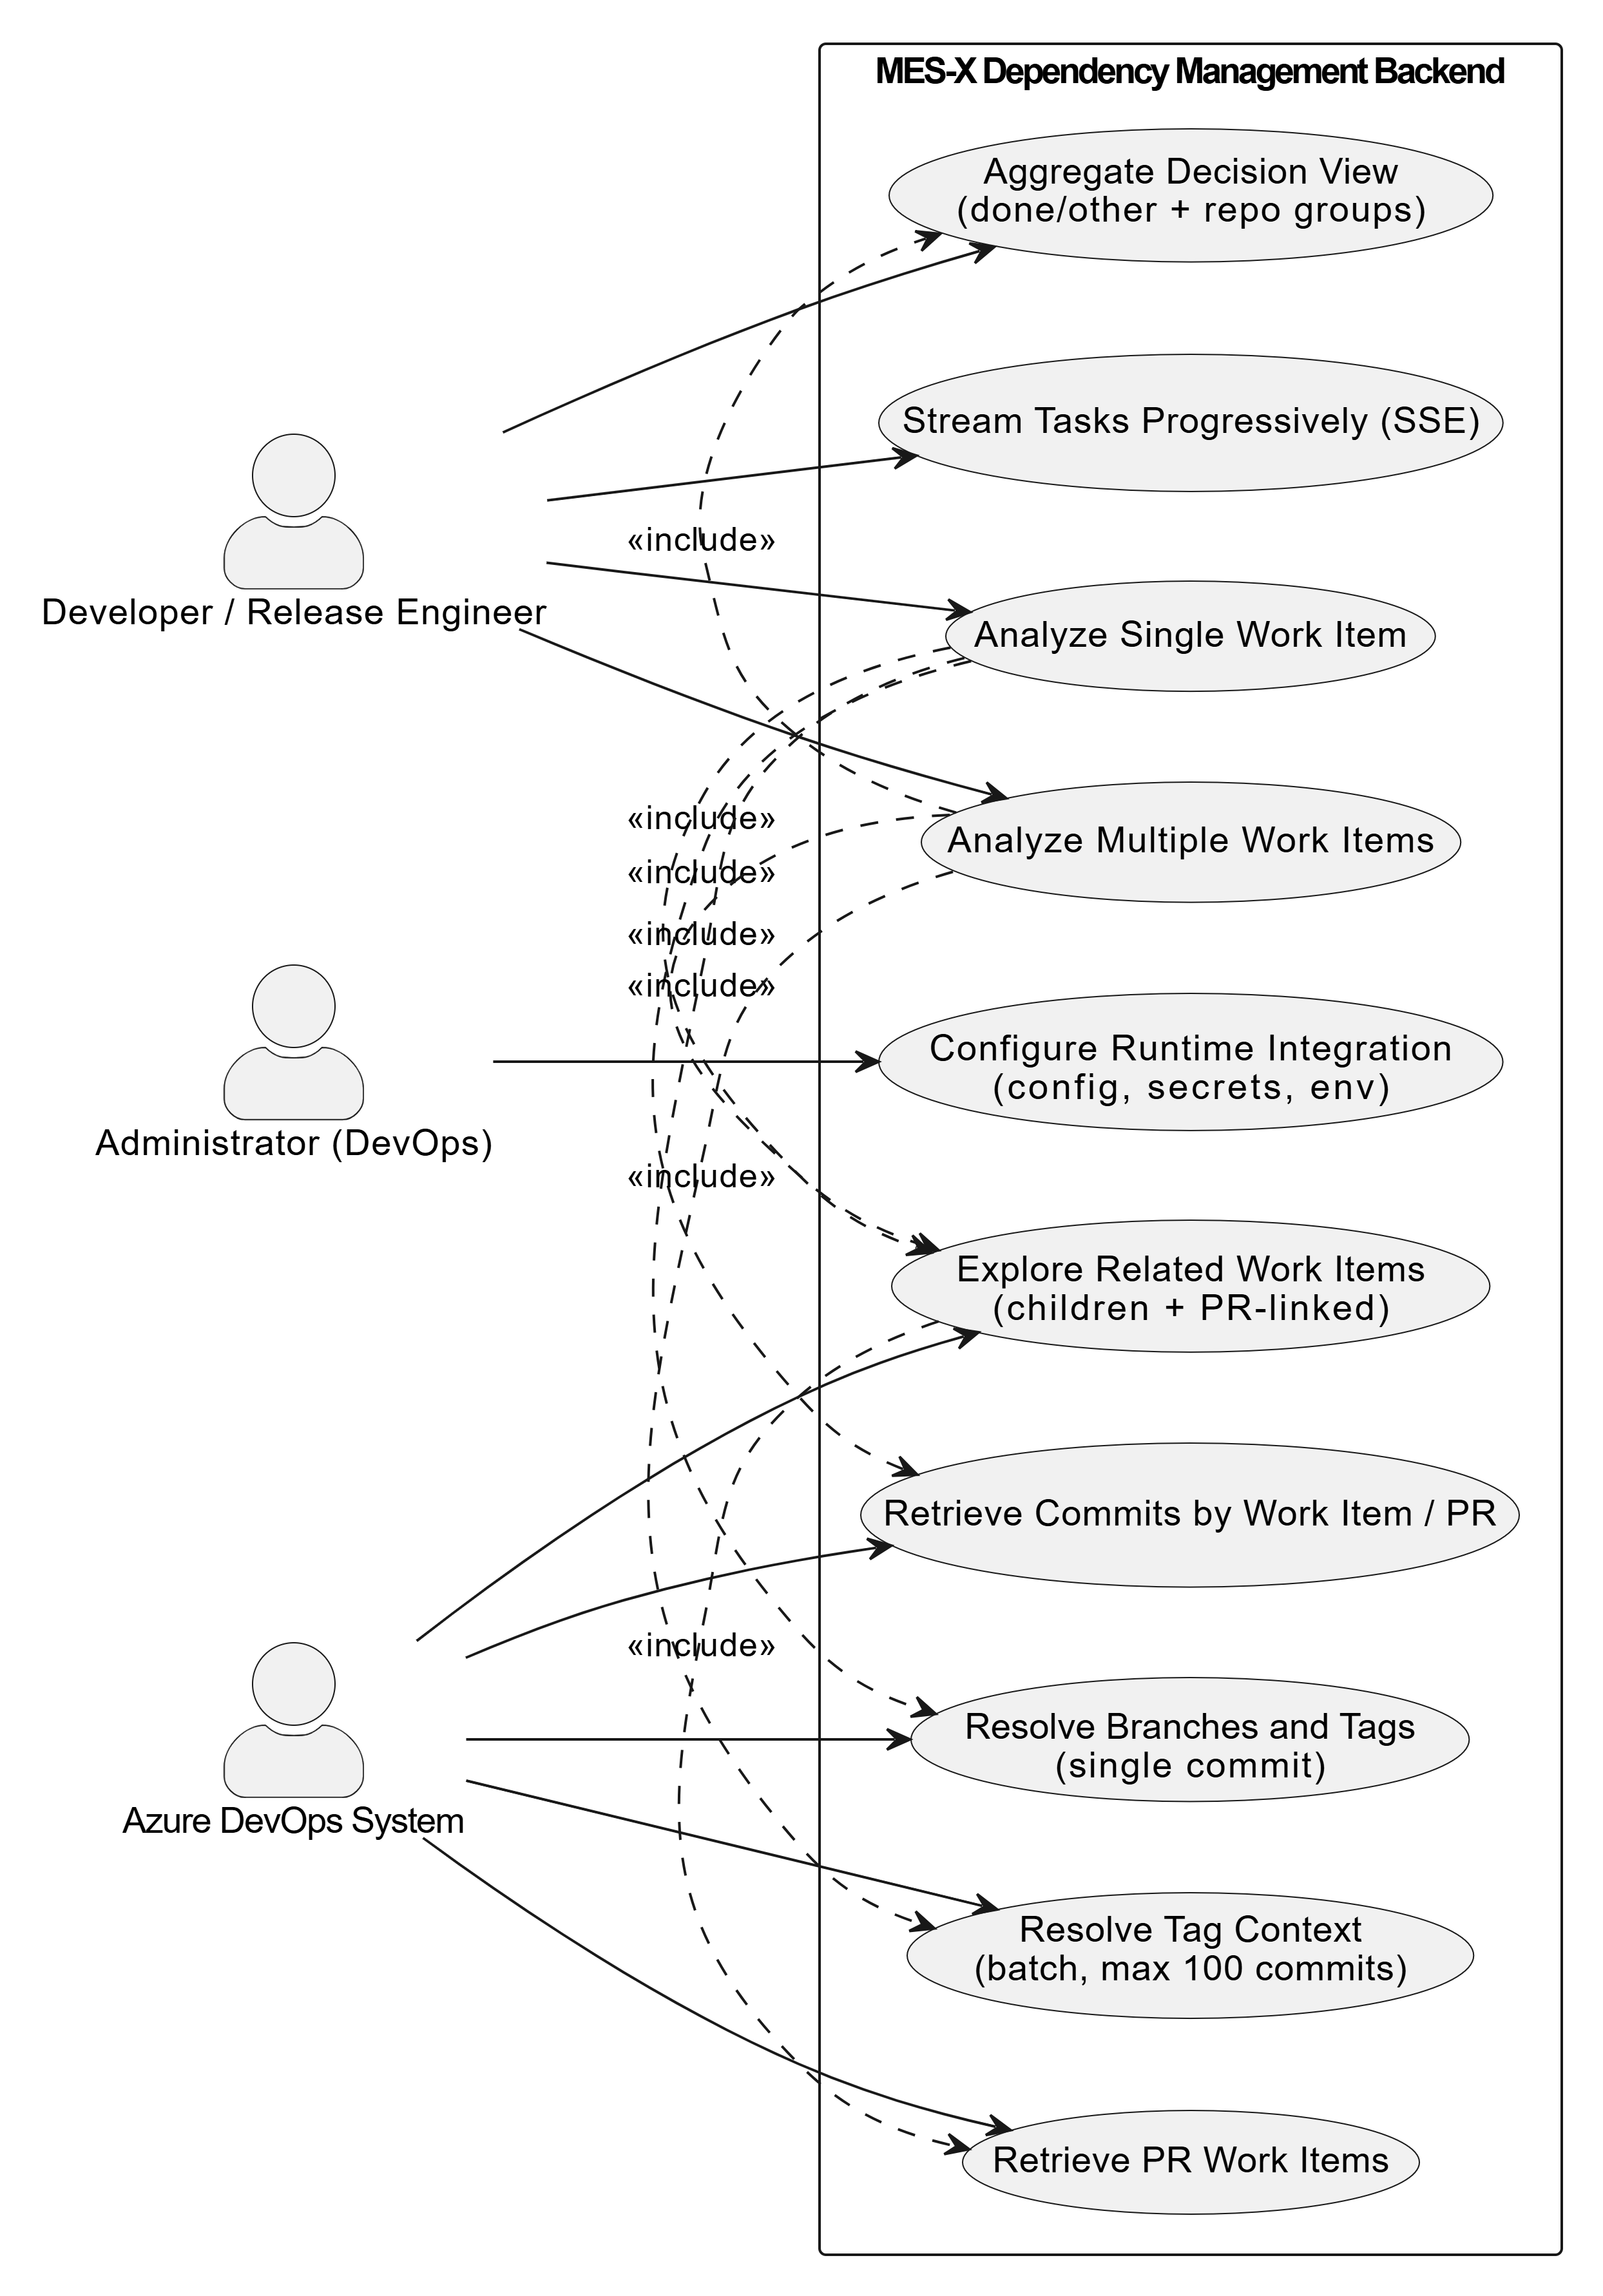
\includegraphics[width=0.92\textwidth,keepaspectratio]{img/archi/use_case.png}
  \caption{Use Case Diagram of the MES-X Dependency Management System.}
  \label{fig:usecase-diagram}
\end{figure}

\subsection{Scope Boundaries}
\label{subsec:scope-boundaries}

Two scope boundaries need to be stated clearly.

First, as established by \textbf{FR-AN-05}, all use cases are read-only. The
system does not create, modify, or delete any artifact in Azure DevOps. It only
retrieves and analyzes existing information, so Azure DevOps appears in the
model only as a data provider.

Second, notification and alerting capabilities, although mentioned in some
internal notes as possible future extensions, are outside the scope of the
current system. This specification covers only the traceability and analysis
capabilities described above.

% ----------------------------------------------------------------------------
\section{Requirements Traceability Summary}
\label{sec:req-traceability}

Table~\ref{tab:req-traceability} summarizes how the functional requirement
groups map to the system components in the proposed architecture. This mapping
creates the link between specification and design and makes it clear which part
of the system is responsible for each requirement set.

\begin{table}[H]
  \centering
  \caption{Functional Requirements to System Component Traceability Matrix}
  \label{tab:req-traceability}
  \begin{tabular}{|p{4.5cm}|p{3cm}|p{5.5cm}|}
    \hline
    \textbf{Requirement Group} & \textbf{Requirement IDs} & \textbf{Addressing Component} \\
    \hline
    Work Item Traceability & FR-WI-01 to FR-WI-06 & Work Item Management Component \\
    \hline
    Pull Request Traceability & FR-PR-01 to FR-PR-04 & Pull Request Resolution Component \\
    \hline
    Commit Traceability & FR-CO-01 to FR-CO-06 & Commit Aggregation Component \\
    \hline
    Data Aggregation & FR-AG-01 to FR-AG-05 & Decision Aggregation Component \\
    \hline
    Analysis and Reporting & FR-AN-01 to FR-AN-05 & All components, Trace UI \\
    \hline
  \end{tabular}
\end{table}

% ----------------------------------------------------------------------------
\section{Conclusion}
\label{sec:req-conclusion}

This chapter defined the requirements for the MES-X Dependency Management
system in a structured and traceable way. The functional requirements cover the
five main capability areas of the solution: work item traceability, pull
request resolution, commit enrichment, data aggregation, and analytical
reporting. The non-functional requirements describe the quality constraints in
the areas of performance, scalability, reliability, maintainability, and
security. The use case model turns those requirements into eleven observable
actor-system interactions.

Together, these requirements form the foundation for the architectural design
that follows.

The next chapter presents the proposed solution and explains the architecture
used to satisfy these requirements, starting with the global three-layer
structure and the four core components of the traceability pipeline.
